\chapter{Mathoden und Techniken}
    \begin{itemize}
        \item Wozu UHV
        \item Oberflächensensetive Methoden
    \end{itemize}
\section{LEED}
    \begin{itemize}
        \item Geometrische Struktur
        \item Mathematische Methoden
    \end{itemize}
\section{PES}
    \begin{itemize}
        \item XPS
        \item UPS
        \item Modele der Anregung
        \item Mittlere Frei weglänge
        \item Integrierte Spektren
    \end{itemize}

\section{ARPES}
    \begin{itemize}
        \item 
    \end{itemize}

\section{Molekül Orbital Tomographie}
    \begin{itemize}
        \item Vereinigung von Experiment und Theorie
        \item MM
    \end{itemize}

    \section{Moment Mikroskopie} \label{sec:MM}
        Bei der Moment Microskopie (\textit{engl.} Momentum Microscopy) ist eine sehr viel versprechende Technik, die für immer mehr Aufsehen in den letzten Jahren gesorgt hat.
        Der größte Vorteil liegt wohl in der Kombination von spektroskopischen Methoden und mikroskopischen Methoden.
        Zuerst wurde dies 1933 durch E. Brüche entdeckt, der eine Zinkplatte mit Hilfe von Photoelektronen und einer magnetischen Linse auf einem Leuchtschirm abbildete \cite{bruche_elektronenmikroskopische_1933}.

        Bei der Moment Mikroskopie ist die zeitgleich Erfassung des polaren und azimuntalen Austrittswinkel von großer Bedeutung. 
        Zusätzlich werden die Elektronen auch nach ihrer kinetsichen Energie sortiert, sodass ein dreidimensionaler Datensatz entsteht.

        \begin{figure}
            \centering
            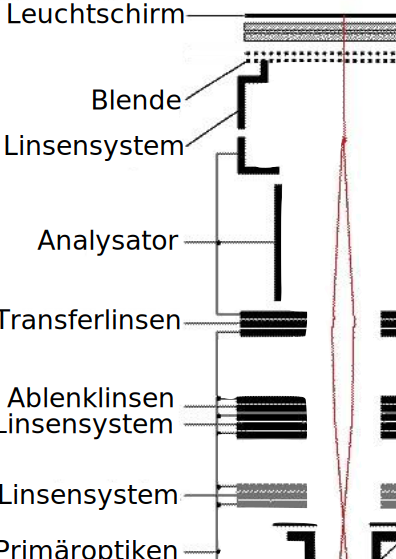
\includegraphics[width=0.7\textwidth]{./content/PEEM_schemaneu.jpg}
            \caption{Exemplarischer Aufbau eines Momentum Microskope. Aus \cite{KUCH}.}
            \label{fig:MM}
        \end{figure}
        Ein exemplarischer Aufbau ist in Abbildung \ref{fig:MM} zu sehen.
        Die durch die Photonen angeregten Elektronen werden durch ein starkes elektrisches Feld von einigen \si{\kilo\volt} von der Probe zum Analysator hin beschleunigt.
        Durch diese große Spannung zwischen Probe und Extraktor ist es möglich ein ein großen Sichtbereich im Impulsraum abzudecken.
        Dies ist nötig, da durch den streifenden Einfall der Photonen und der Abberation der elektrostatischen Linsen nur einen kleinen Akzeptanzwinkel zur Verfügung stehen würde. \textbf{QUELLE}
        Wichtig bei der Kathoden Linse ist, dass das Feld zwischen Probe und Linse sehr homogen ist, damit der Austrittswinkel erhalten bleibt.
        Anschließend werden die Elektronen durch elektrostatische Linsen fokusiert.
        Mit Hilfe von Kontrastblenden kann dann eine Auflößung von einigen \si{\nano\meter} erreicht werden. \textbf{QUELLE}.
        Hierbei gibt es an zwei verschiedenen Stellen Blenden, je nach dem ob im Realraum oder im Impulsraum ein Bild aufgenommen werden soll.

        \begin{figure}
            \centering
            \includegraphics[width=0.7\textwidth]{./content/Real_k.PNG}
            \caption{Die verschiedenen Konfiguration der Blenden um zwischen realraum Bild und Impulsraum Bild umzuschalten. Aus \cite{Focus}.}
            \label{fig:real_k}
        \end{figure}
        Für den Impulsraum ist dies in Abbildung \ref{fig:real_k}\,a und für den Realraum in Abbildung \ref{fig:real_k}\,b dargestellt.
        Um ein Bild im Realraum zu erhalten muss die Blende im Brennpunkt eingesetzt sein, auf dem Eintrittsspalt des Energyanalysators wird dann das Bild der Oberfläche projeziert.
        Wird hingegen in der ersten Bildebene die Blende eingesetzt so wird auf dem Eintrittsspalt das Beugungsbild abgebildet. 
        Die restlichen Linsen, Stigmatoren und Ablenker sind dafür da, dass Bild zu zentrieren und Abberation auszugleichen.

        Als Energiealysator kommt ein hemisphärischer Analysator zum Einsatz, für gepulste Photonenquellen würde sich auch ein \textit{Time of flight - TOF} (Flugzeit) Analysator eignen.
        Bei dem hemisphärischer Analysator werden die Elektronen zwischen zwei Halbkugeln durch ein statisches elektrisch Feld auf eine Kreisbahn gezwungne.
        Dabei ist das Feld so gewählt, dass nur die mit der richtigen kinetischen Energie eintretenden Elektronen auch auf den Austrittsspalt abgebildet werden.
        Bei einem TOF Analysators wird die kinetische Energie aus der Flugzeit der Elektronen bestimmt, weswegen es nur für gepulste Photonenquellen möglich ist.

        Nach dem Energiealysator gibt es nochmal ein paar Optiken, die das Bild auf den Detektor abbilden.
        Bei dem Detektor handelt es sich um eine C-MOS Kamera die das Bild der auf den Leuchtschirm auftreffenden Elektronen aufnimmt.
        



        \begin{figure}
            \centering
            \includegraphics[width=0.7\textwidth]{./content/MM.png}
            \caption{Der für die durchgeführten Experimente verwendete Aufbau.}
            \label{fig:aufbau}
        \end{figure}
        Der gesamte Aufbau aus dem PEEM und der Präperationskammer ist in Abbildung \ref{fig:aufbau} zu finden.

        \begin{itemize}
            \item Erweiterung auf Spinaufgelöst möglich
            \item TOF
            \item Zeitaufgelöst
            \item Real und Impulsraum
        \end{itemize}

    \section{Molekül Orbital Tomographie}
        Die Molekühle Orbital Tomographie vereinigt nun die Vorteile des Momentum Mikroskopes mit der Theorie der Dichtefunktionaltheorie (DFT) um Molekühlorbitale zu identifizieren.


